\documentclass{beamer}

\usepackage[utf8]{inputenc}
\usepackage[english]{babel}
\usepackage{textpos}
\usepackage{graphicx}
\usepackage{textcomp}
\usepackage{animate}
\usepackage{comment}
%\usepackage{multicol}
%\setlength{\columnsep}{5cm}
\usepackage{amsmath}
\usepackage{amsfonts}
\usepackage{verbatim}
\usepackage{varwidth}
\usepackage{caption}
\usepackage{dcolumn}
\usepackage{amssymb}
\usepackage{algorithm}
\usepackage{algorithmic}
%\usepackage{physics}
\usepackage{hyperref}
\usepackage{scalerel,stackengine}
\usepackage{fancyvrb}


\newcommand{\code}[1]{\texttt{#1}}
\newcommand{\shp}{$>>>$ }
\newcommand{\tab}{\hspace*{22pt}}

\usetheme{Madrid}

\title{Chapter 3: \\ Some Simple Numeric Programs}
\author{EEC 3150}
\date{}

\institute{Trevecca Nazarene University}
 


%%%%%%%%% BEGIN DOCUMENT %%%%%%%%%
%%%%%%%%% BEGIN DOCUMENT %%%%%%%%%
%%%%%%%%% BEGIN DOCUMENT %%%%%%%%%

\begin{document}

% get title page 
\frame{\titlepage}
 
%%%%%%%%%%
%%%%%%%%%%
\begin{frame}	
	\frametitle{Outline}
	\tableofcontents	
\end{frame}


%%%%%%%%%%
%%%%%%%%%%
\section{Exhuastive Enumeration (Brute Force)}

\begin{frame}	
	\center{\Huge{Exhuastive Enumeration \\ \vspace{5pt} (Brute Force)}}
\end{frame}

\begin{frame}	
	\frametitle{Exhuastive Enumeration (Brute Force)}
	
	\begin{alertblock}{Exhuastive enumeration (brute force):}
		\textbf{Exhuastive enumeration} (more commonly \textbf{brute force}) is an approach to problem-solving which naively tests every possible solution to a problem
		
		\vspace{5pt}
		
		Pros:
		\begin{itemize}
			\item Easy to implement and understand
			\item For simple problems, computers are fast enough
		\end{itemize}
		
		\vspace{5pt}
		
		Cons:
		\begin{itemize}
			\item For some problems, the space of possible solutions is enormous and exploring all of them is intractable for even a billion supercomputers working together
		\end{itemize}
		
		\vspace{5pt}
		
		For which problem is brute force a better fit?
		\begin{itemize}
			\item Guessing someone's 4-digit PIN
			\item Finding the maximum value of a real-valued function of 100 variables
		\end{itemize}
	\end{alertblock}
	
\end{frame}

\begin{frame}	
	\frametitle{Exhuastive Enumeration (Brute Force)}
	
	\begin{block}{Code example:}
		\minipage{0.5\textwidth}
			Find the cube root of a perfect cube
			
			\vspace{10pt}
			
			\begin{scriptsize}
			\code{x = 64 \\[-5pt]
			ans = 0 \\[-5pt]
			\tab \\[-5pt]
			while ans**3 < abs(x): \\[-5pt]
			\tab ans = ans + 1 \\[-5pt]
			\#end \\[-5pt]
			\tab \\[-5pt]
			if ans**3 != abs(x): \\[-5pt]
			\tab print(x, 'is not a perfect cube') \\[-5pt]
			else: \\[-5pt]
			\tab if x < 0: \\[-5pt]
			\tab \tab ans = -ans \\[-5pt]
			\tab \#end \\[-5pt]
			\tab print('Cube root of', x,'is', ans) \\[-5pt]
			\#end
			}
			\end{scriptsize}
		\endminipage\hfill
		\minipage{0.5\textwidth}
			\begin{itemize}
				\item Common coding strategy: start with an initial guess at a solution (\code{ans=0}) then use a loop to iterate through other possible solutions
				\item Code tests ALL possible solutions until it either finds the solution or has eliminated all possible solutions
				\item How to know all possible solutions have been elinimated?
				\item While loop stopping condition?
			\end{itemize}
		\endminipage\hfill
	\end{block}
	
\end{frame}

\begin{frame}	
	\frametitle{Exhuastive Enumeration (Brute Force)}
	
	\begin{block}{Code example:}
		\minipage{0.55\textwidth}
			Guess someone's 4-digit PIN (0-9) by listing all possible PINs
			
			\vspace{10pt}
			
			\begin{scriptsize}
			\code{for a in range(10): \\[-5pt]
			\tab for b in range(10): \\[-5pt]
			\tab \tab for c in range(10): \\[-5pt]
			\tab \tab \tab for d in range(10): \\[-5pt]
			\tab \tab \tab \tab print( str(a)+str(b)+ \\[-5pt]
			\tab \tab \tab \tab \tab str(c)+str(d) )
			}
			\end{scriptsize}
		\endminipage\hfill
		\minipage{0.45\textwidth}
			\begin{itemize}
				\item List all 10 possible choices for each of the 4 digits
				\item Use \code{range(10)} to generate integers
				\item Use \code{str()} to take advantage of string concatenation (+)
				\item Best case: first guess
				\item Worst case: last guess (10,000)
				\item Average case: 10,000/2 = 5,000
			\end{itemize}
		\endminipage\hfill
	\end{block}
	
\end{frame}

\begin{frame}	
	\frametitle{Approximate Solutions and Brute Force}
	
	\begin{alertblock}{Approximate solutions:}
		Problem: find the square root of any non-negative number
		
		\vspace{10pt}
		
		Issue with the problem statement:
		\begin{itemize}
			\item Square root of 2 is irrational, requires infinite digits
			\item Computers have a finite level of precision (number of digits) and could only give an approximate value
		\end{itemize}
		
		\vspace{10pt}
		
		Better problem statement:
		\begin{itemize}
			\item Approximate the square root of any non-negative number with a precision of $\epsilon$
		\end{itemize}
	\end{alertblock}
	
\end{frame}

\begin{frame}	
	\frametitle{Approximate Solutions and Brute Force}
	
	\begin{block}{Example:}
		\minipage{0.58\textwidth}
			Approximate the square root of $x$ to within a precision of $\epsilon$
			
			\vspace{5pt}
			
			\begin{scriptsize}
			\code{x = 100 \\[-5pt]
			\tab \\[-5pt]
			eps = 0.01 \\[-5pt]
			step    = 0.001 \\[-5pt]
			ans     = 0.0 \\[-5pt]
			\tab \\[-5pt]
			while abs(ans**2 - x) $>$= eps and ans**2 $<$= x: \\[-5pt]
			\tab ans += step \\[-5pt]
			\#end \\[-5pt]
			\tab \\[-5pt]
			if abs(ans**2 - x) $>$= eps: \\[-5pt]
			\tab print('Failed on square root of', x) \\[-5pt]
			else: \\[-5pt]
			\tab print('sqrt(',x,') is approx.', ans) \\[-5pt]
			\#end
			}
			\end{scriptsize}
		\endminipage\hfill
		\minipage{0.42\textwidth}
			\begin{itemize}
				\item Initial guess \code{ans = 0.0}
				\item Checks whether \code{ans} is a solution or is beyond the scope of possible solutions (while loop condition)
				\item Until the while loop is done, it increments \code{ans} by \code{step} at each iteration
			\end{itemize}
		\endminipage\hfill
		
		\vspace{10pt}
		
		Question: What happens if the step size is too big?
	\end{block}
	
\end{frame}

\begin{frame}	
	\frametitle{Approximate Solutions and Brute Force}
	
	\begin{block}{Example:}
		Approximate the square root of $x$ to within a precision of $\epsilon$
		
		\begin{figure}[ht]
			\centering
			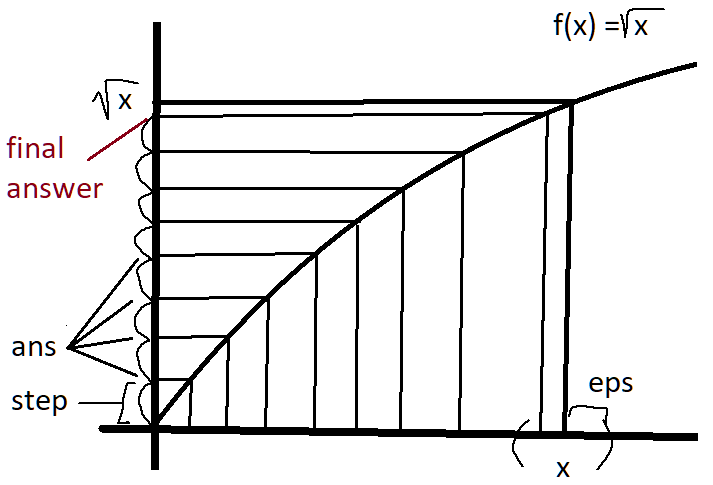
\includegraphics[width=0.73\linewidth]{ExhaustiveSquareRoot}
			\caption{Visual depiction of the algorithm}
		\end{figure}
	\end{block}
	
\end{frame}

%%%%%%%%%%
%%%%%%%%%%
\section{The Bisection Method}

\begin{frame}	
	\center{\Huge{The Bisection Method}}
\end{frame}

\begin{frame}	
	\frametitle{Approximate Solutions and the Bisection Method}
	
	\begin{block}{Motivating the bisection method:}
		We almost always want better algorithms than naive brute force approaches
		
		\vspace{10pt}
		
		Consider the problem of looking up \emph{median} in the dictionary:
		\begin{itemize}
			\item The dumb way (brute force): start at the beginning and look at every word until we find it
			\item The smart way: \\
					1. \emph{The words are all sorted alphabetically} \\
					2. Guess a page that you think is close \\
					3. If the page contains words before \emph{median}, you need to flip futher ahead (or vice versa) \\
					4. Keep guessing closer and closer pages until you arrive at the correct page
		\end{itemize}
	\end{block}
	
\end{frame}

\begin{frame}	
	\frametitle{Approximate Solutions and the Bisection Method}
	
	\begin{block}{Motivating the bisection method:}
		Look up \emph{median} in the dictionary:
		
		\begin{figure}[ht]
			\centering
			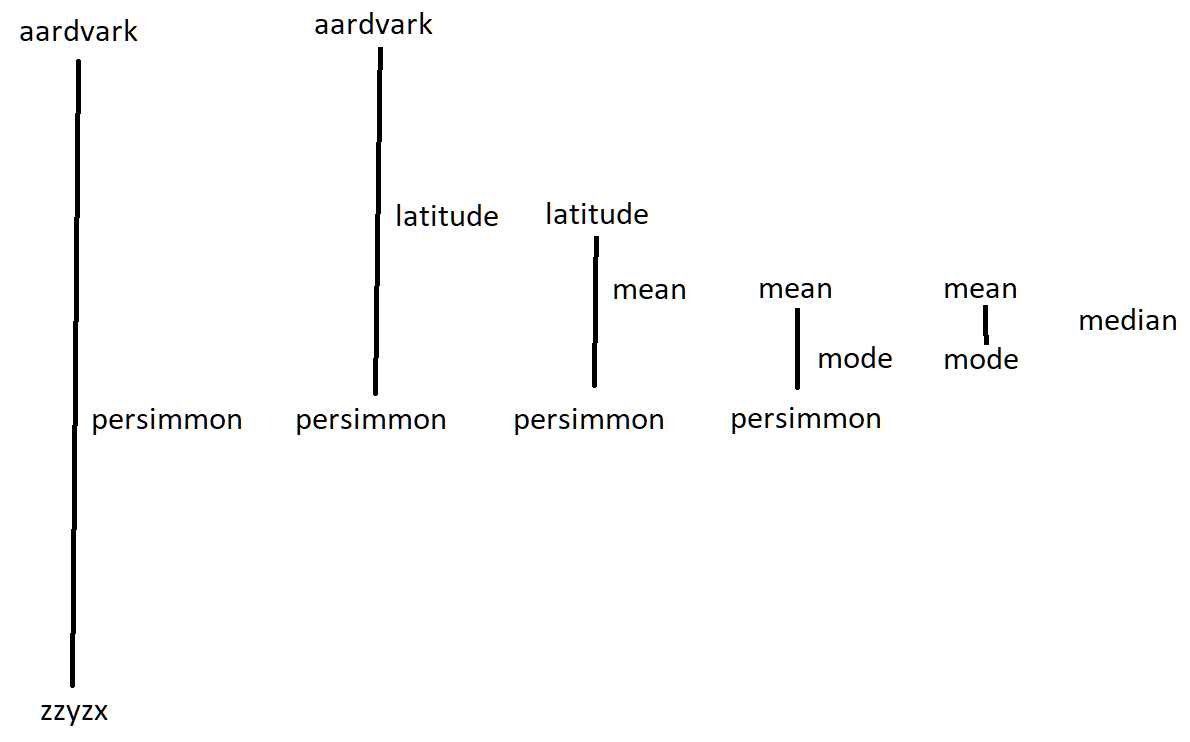
\includegraphics[width=0.73\linewidth]{DictionaryBisection}
			\caption{Visual depiction of the algorithm}
		\end{figure}
	\end{block}
	
\end{frame}

\begin{frame}	
	\frametitle{Approximate Solutions and the Bisection Method}
	
	\begin{block}{Example:}
		\minipage{0.5\textwidth}
			Approximate the square root of $y$ \\ to within a precision of $\epsilon$
			
			\vspace{5pt}
			
			\begin{scriptsize}
			\code{y = 10 \\[-5pt]
			\tab \\[-5pt]
			eps = 0.01 \\[-5pt]
			low = 0.0 \\[-5pt]
			high = max(1.0, y) \\[-5pt]
			ans = (high + low)/2 \\[-5pt]
			\tab \\[-5pt]
			while abs(ans**2 - y) $>$= eps: \\[-5pt]
			\tab if ans**2 $<$ y: \\[-5pt]
			\tab \tab low = ans \\[-5pt]
			\tab else: \\[-5pt]
			\tab \tab high = ans \\[-5pt]
			\tab \#end \\[-5pt]
			\tab \\[-5pt]
			\tab ans = (high + low)/2 \\[-5pt]
			\#end \\[-5pt]
			\tab \\[-5pt]
			print('sqrt(',y,') is approx.', ans) 
			}
			\end{scriptsize}
		\endminipage\hfill
		\minipage{0.5\textwidth}
			Solve $f(x) = x^2 - y = 0$, \\ where y = 10
			\vspace{8pt}
			\begin{itemize}
				\item Make sure that the real answer is between your initial \code{low, high} guesses
				\item At each step, your new \code{ans} guess should be somewhere in between \code{low,high} (the mean is the easiest solution)
				\item Re-assign the value of \code{low} or \code{high} depending on whether \code{ans} was above or below the real answer
			\end{itemize}
		\endminipage\hfill
	\end{block}
	
\end{frame}

\begin{frame}	
	\frametitle{Approximate Solutions and the Bisection Method}
	
	\begin{block}{Motivating the bisection method:}
		Approximate $\sqrt{10}$ with the bisection method:
		
		\begin{figure}[ht]
			\centering
			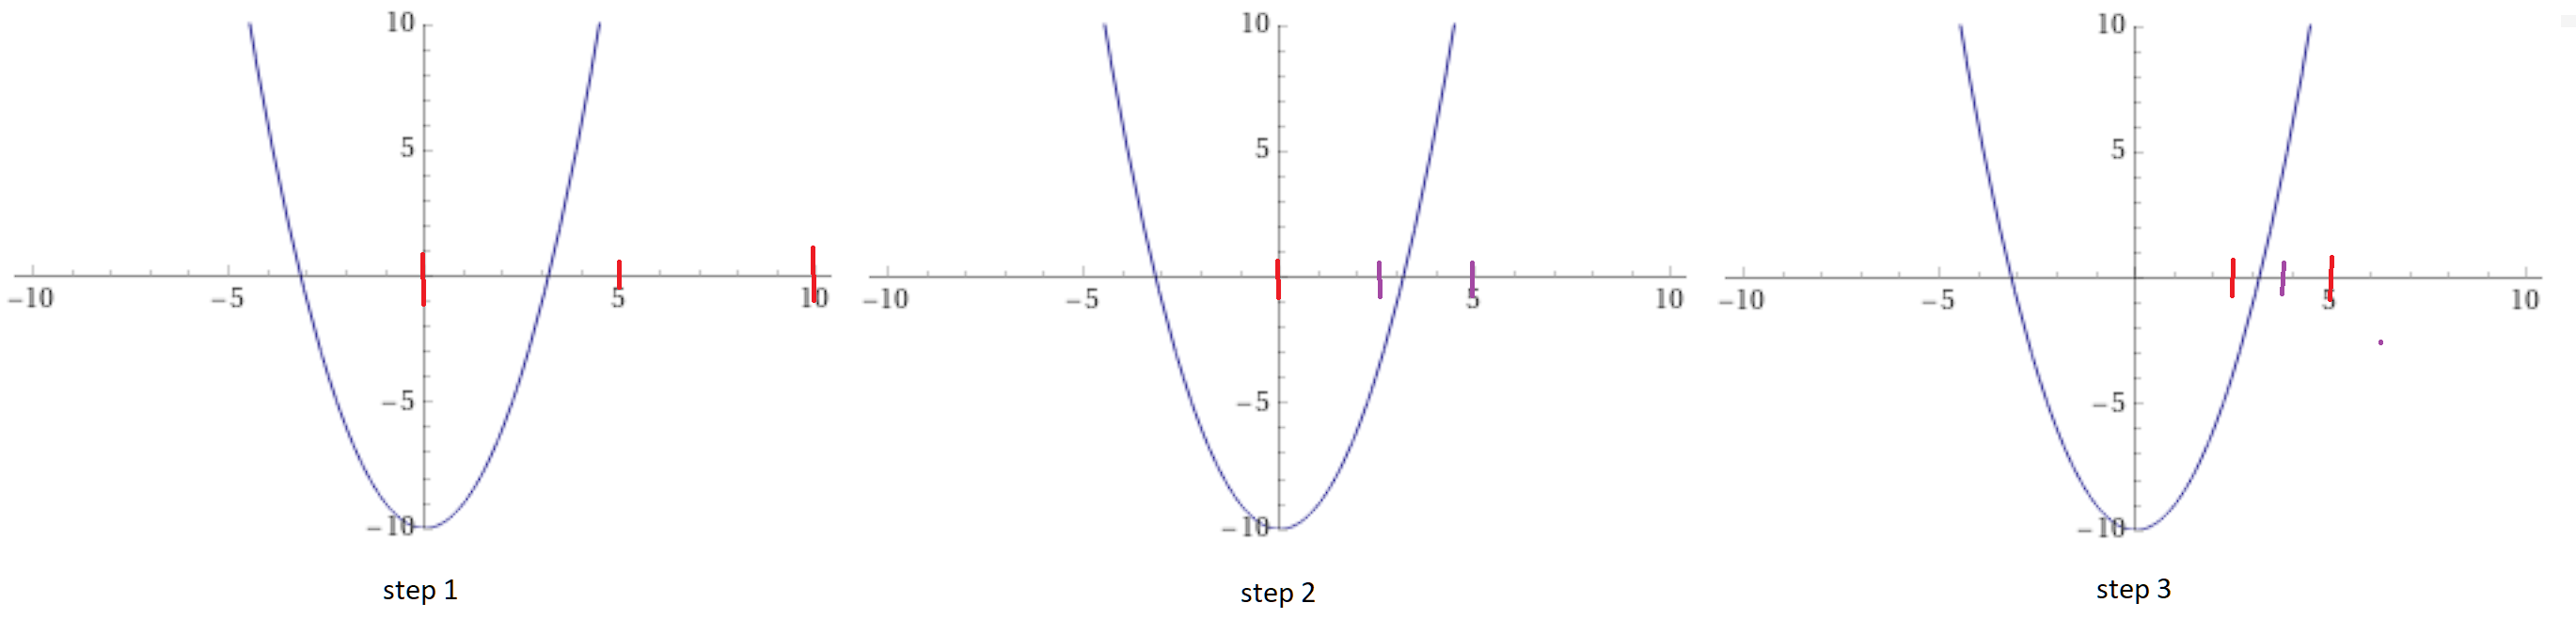
\includegraphics[width=0.99\linewidth]{BisectionSquareRoot}
			\caption{Visual depiction of the algorithm}
		\end{figure}
	\end{block}
	
\end{frame}


%%%%%%%%%%
%%%%%%%%%%
\section{Floating-Point Arithmetic}

\begin{frame}	
	\center{\Huge{Floating-Point Arithmetic}}
\end{frame}



\begin{frame}	
	\frametitle{Approximate Solutions and the Bisection Method}
	
	\begin{block}{Question:}
			What do you expect the follow code to print?
			
			\vspace{5pt}
			
			\code{total = 0.0 \\
			for i in range(15): \\
		    \tab total += 0.1 \\
		    \tab print(total)
			}
			
	\end{block}
	
\end{frame}

\begin{frame}	
	\frametitle{Floating-Point Arithmetic}
	
	\begin{block}{Example:}
		\minipage{0.5\textwidth}
			We get
			
			\vspace{5pt}
			
			\begin{scriptsize}
			\code{0 \\[-5pt]
			0.1 \\[-5pt]
			0.2 \\[-5pt]
			0.30000000000000004 \\[-5pt]
			0.4 \\[-5pt]
			0.5 \\[-5pt]
			0.6 \\[-5pt]
			0.7 \\[-5pt]
			0.7999999999999999 \\[-5pt]
			0.8999999999999999 \\[-5pt]
			0.9999999999999999 \\[-5pt] 
			1.0999999999999999 \\[-5pt]
			1.2 \\[-5pt]
			1.3 \\[-5pt]
			1.4000000000000001 \\[-5pt]
			1.5000000000000002
			}
			\end{scriptsize}
		\endminipage\hfill
		\minipage{0.5\textwidth}
			Why?
			\vspace{8pt}
			\begin{itemize}
				\item In computers, numbers are represented as a binary format instead of decimal format
				\item Computers only have a finite level of precision for numbers (i.e., number of digits)
				\item 0.1 cannot be represented exactly with a finite number of digits in binary
				\item Repeatedly adding it accumulates errors
			\end{itemize}
		\endminipage\hfill
		
		\vspace{10pt}
		
		Why can't 0.1 be represented exactly in binary???
	\end{block}
	
\end{frame}

\begin{frame}	
	\frametitle{Floating-Point Arithmetic}
	
	\begin{block}{Number representation in decimal format:}
		In decimal format, numbers are represented as a sum of multiples of powers of 10 (the base of the decimal system)
		\begin{equation*}
			\begin{split}
				123.4 	& = 100 + 20 + 3 + 0.4\\
						& = 1\cdot100 + 2\cdot 10+3\cdot1 + 4\cdot0.1 \\
						& = 1\cdot10^2 + 2\cdot10^1+3\cdot10^0 + 4\cdot10^{-1}\\
						& = \sum_{i=-1}^2 d_i \cdot 10^i
			\end{split}
		\end{equation*}
		where $d_{-1}=4, d_0=3, d_1=2,d_2=1$
		
		\vspace{10pt}
		
		Also, in scientific notation, $123.4 = 1.234\cdot10^{-2}$
	\end{block}
	
\end{frame}

\begin{frame}	
	\frametitle{Floating-Point Arithmetic}
	
	\begin{block}{Number representation in decimal format:}
		Inspired by scientific notation, we could choose to represent this number as just a list of digits and an exponent (this is how floating-point systems work):
		
		\vspace{10pt}
		This assumes that we know that the base of this system (in the decimal case, 10)
		\begin{itemize}
			\item All digits must be integers between 0-9 (can't be 10 or greater)
			\item Use powers of 10 to reconstruct the number
		\end{itemize}
		
		\vspace{10pt}
		$(1234, 2) \rightarrow 1.234\cdot10^{2} = 1\cdot10^2 + 2\cdot10^1+3\cdot10^0 + 4\cdot10^{-1} = 123.4$
		
		\vspace{10pt}
		(NOTE: I'm using the convention of Section 1.3 in Heath, not 3.3 in Guttag)
	\end{block}
	
\end{frame}

\begin{frame}	
	\frametitle{Floating-Point Arithmetic}
	
	\begin{block}{Number representation in binary format:}
		We can use whatever base we want (base 2 is binary)
		
		\vspace{10pt}
		
		\begin{itemize}
			\item All digits must be integers 0, 1
			\item Use powers of 2 to reconstruct the number
		\end{itemize}
		
		\vspace{10pt}
		$(10011, 2) \rightarrow 1.0011\cdot2^{2} = 1\cdot2^2 + 0\cdot2^1+0\cdot2^0 + 1\cdot2^{-1} +1\cdot2^{-2} = 100.11_2$ \\
		$\hspace{114pt} = 1\cdot4 + 0\cdot2+0\cdot1 + 1\cdot\frac{1}{2} +1\cdot\frac{1}{4} = 4.75_{10}$
		
		\vspace{10pt}
		Conversion from binary to decimal: $100.11_2 = $
	\end{block}
	
\end{frame}

\begin{frame}	
	\frametitle{Floating-Point Arithmetic}
	
	\begin{alertblock}{Defm: floating-point system:}
%		A floating-point system for representing numbers is defined as follows:
		
%		\vspace{10pt}
		
		\minipage{0.48\textwidth}
			Define the following integers:
			\begin{itemize}
				\item $b$: the base (use powers of this number)
				\item $p$: the precision (how many digits)
				\item $L,U$: the lower and upper limits of the exponent
			\end{itemize}
			
			\vspace{10pt}
			
			Floating-point numbers have two parts:
			\begin{itemize}
				\item The \emph{mantissa}: $d_0d_1d_2\cdots d_{p-1}$
				\item The \emph{exponent}: $E$
			\end{itemize}
		\endminipage\hfill		
		\minipage{0.04\textwidth}
		\endminipage\hfill		
		\minipage{0.48\textwidth}
			Then, any \textbf{floating-point number} $x\in\mathbb{F}$ has the form		
			\begin{equation*}
				x = \pm b^E \cdot\sum_{i=0}^{p-1} \frac{d_i}{b^i}
			\end{equation*}
			where all the $d_i$'s are integers such that
			\begin{equation*}
				0 \le d_i < b, \quad i = 0, \cdots, p-1
			\end{equation*}
			and $E$ is an integer such that
			\begin{equation*}
				L \le E \le U
			\end{equation*}
		\endminipage\hfill
	\end{alertblock}
	
\end{frame}

\begin{frame}	
	\frametitle{Floating-Point Arithmetic}
	
	\begin{block}{Examples:}
		\begin{equation*}
			x = \pm b^E \cdot\sum_{i=0}^{p-1} \frac{d_i}{b^i}
		\end{equation*}
		
%		\vspace{10pt}
		
		Decimal ($p=4$):
		
		\vspace{10pt}
		$123.4_{10} = 10^2 \cdot \Big(\frac{1}{10^0}+\frac{2}{10^1}+\frac{3}{10^2}+\frac{4}{10^3}\Big) = (1234,2)$
		
		\vspace{10pt}
		
		Decimal ($p=6$):
		
		\vspace{10pt}
		$123.400_{10} = 10^2 \cdot \Big(\frac{1}{10^0}+\frac{2}{10^1}+\frac{3}{10^2}+\frac{4}{10^3}+\frac{0}{10^4}+\frac{0}{10^5}\Big) = (123400,2)$
		
		\vspace{10pt}		
		Obviously, 123.4 and 123.400 represent the same value, but the 6-digit system can represent numbers that the 4-digit system cannot: e.g., 123.41
	\end{block}
	
\end{frame}

\begin{frame}	
	\frametitle{Floating-Point Arithmetic}
	
	\begin{block}{Examples:}
		\begin{equation*}
			x = \pm b^E \cdot\sum_{i=0}^{p-1} \frac{d_i}{b^i}
		\end{equation*}
		
%		\vspace{10pt}
		
		Binary ($p=5$):
		
		\vspace{10pt}
		$100.11_{2} = 2^2 \cdot \Big(\frac{1}{2^0}+\frac{0}{2^1}+\frac{0}{2^2}+\frac{1}{2^3}+\frac{1}{2^4}\Big) = (10011,2)$
		
		\vspace{10pt}
		
		Binary ($p=8$):
		
		\vspace{10pt}
		$100.1100_{2} = 2^2 \cdot \Big(\frac{1}{2^0}+\frac{0}{2^1}+\frac{0}{2^2}+\frac{1}{2^3}+\frac{1}{2^4}+\frac{0}{2^5}+\frac{0}{2^6}+\frac{0}{2^7}\Big) = (1001100,2)$
		
		\vspace{10pt}		
		Again, these are the same values, but the second system can represent more numbers
	\end{block}
	
\end{frame}

\begin{frame}	
	\frametitle{Floating-Point Arithmetic}
	
	\begin{alertblock}{Properties of floating-point systems:}
		Special numbers:
		\begin{itemize}
			\item Total numbers possible: \\
					$2(b-1)b^{p-1}(U-L+1)+1$
			\item \textbf{Underflow limit} (UFL): The smallest possible number that can be represented by a floating point system: \\
					UFL = $b^L$
			\item \textbf{Overflow limit} (UFL): The largest possible number that can be represented by a floating point system: \\
					OFL = $b^{U+1}(1-b^{-p})$
			\item \textbf{Machine precision} ($\epsilon_{mach}$): : \\ The smallest possible relative error between a real number and its float representation, or, the smallest possible relative difference bewteen two floats:
					$\epsilon_{mach} = b^{1-p}, \frac{1}{2} b^{1-p}$ (depends on how the computer rounds numbers)
		\end{itemize}
	\end{alertblock}
	
\end{frame}

\begin{frame}	
	\frametitle{Floating-Point Arithmetic}
	
	\begin{figure}[ht]
		\centering
		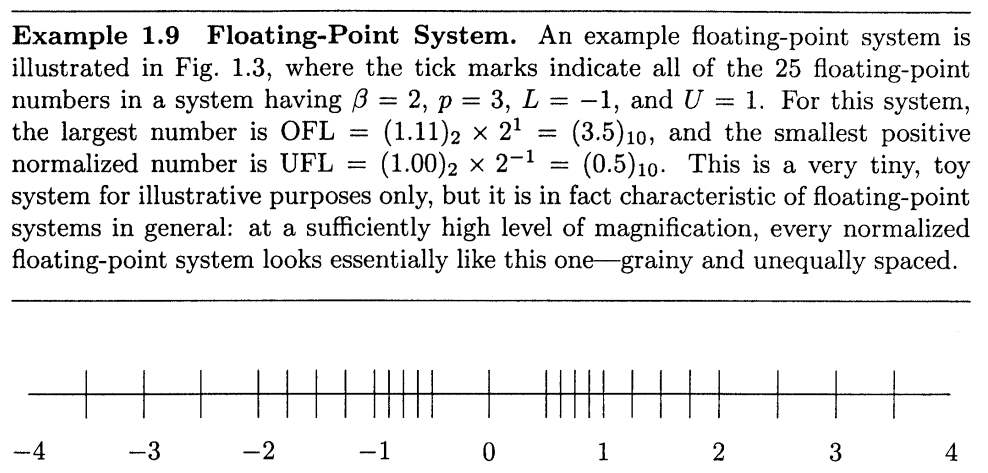
\includegraphics[width=0.99\linewidth]{HeathFloatingPoint}
		\caption{Example floating-point system (Heath)}
	\end{figure}
	
\end{frame}

\begin{frame}	
	\frametitle{Floating-Point Arithmetic}
	
		\minipage{0.48\textwidth}
			Try to construct 7 in binary:
			\begin{itemize}
				\item Left to right: 8's place, 4's place, 2's place, 1's place
				\item Put a 1 in the largest digit's that isn't larger than 7 (i.e., 4)
				\item 3 remainder
				\item Put a 1 in the largest digit's that isn't larger than 3 (i.e., 2)
				\item 1 remainder
				\item Put a 1 in the largest digit's that isn't larger than 1 (i.e., 1)
				\item Done: $7_{10}=0111_2$
			\end{itemize}
		\endminipage\hfill		
		\minipage{0.04\textwidth}
		\endminipage\hfill		
		\minipage{0.48\textwidth}
			\begin{figure}[ht]
				\centering
				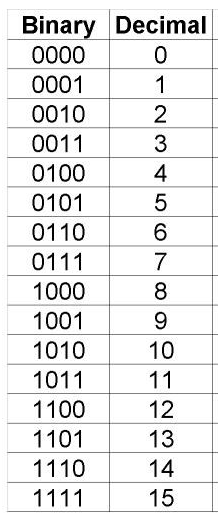
\includegraphics[width=0.54\linewidth]{BinaryDecimalChart}
%				\caption{Visual depiction of the algorithm}
			\end{figure}
		\endminipage\hfill
	
\end{frame}


\begin{frame}	
	\frametitle{Floating-Point Arithmetic}
	
	\begin{block}{Example:}
		Finally, let's try to construct 0.1 in binary
			
		\vspace{5pt}
		\minipage{0.5\textwidth}
			\begin{scriptsize}
			\code{x = 0.1 \\[-5pt]
			\tab \\[-5pt]
			n = 20 \\[-5pt]
			total = 0.0 \\[-5pt]
			binary = '0.' \\[-5pt]
			for i in range(1,n): \\[-5pt]
			\tab test = total + 2**(-i) \\[-5pt]
    			\tab if test < x: \\[-5pt]
			\tab \tab total = test \\[-5pt]
			\tab \tab binary +='1' \\[-5pt]
			\tab else: \\[-5pt]
			\tab \tab binary += '0' \\[-5pt]
			\tab \# end \\[-5pt]
			\# end \\[-5pt]
			print(x, total, binary)
			}
			\end{scriptsize}
		\endminipage\hfill
		\minipage{0.5\textwidth}
			\begin{itemize}
				\item Left to right: 1's place, 1/2's place, 1/4's place, etc.
				\item Put a 1 in the largest digit's that isn't larger than 0.1 (or its remainder at later steps)
			\end{itemize}
		\endminipage\hfill
	\end{block}
	
\end{frame}

\begin{frame}	
	\frametitle{Floating-Point Arithmetic}
	
	\begin{block}{Conclusion:}
		0.1 is an infinitely repeating binary expansion (much like 1/3 is in decimal form)
	\end{block}
	
\end{frame}

%%%%%%%%%%
%%%%%%%%%%
\section{The Newton-Raphson Method}

\begin{frame}	
	\center{\Huge{The Newton-Raphson Method}}
\end{frame}

\begin{frame}	
	\frametitle{The Newton-Raphson Method}
	
	\begin{alertblock}{Defn: Newton-Raphson:}
		\begin{itemize}
			\item Moving from brute force to bisection was an improvement because we were able to incorporate additional knowledge about the search space: that it was sorted/ordered
			\item We can continue to make more efficient methods by utilizing more information about the search space
		\end{itemize}
		
		\vspace{5pt}
		
		The \textbf{Newton-Raphson method} is an algorithm specifically designed to find roots of real-valued functions which utilizes the derivative of the function
		
		\vspace{5pt}
		
		Starting with some initial guess at a solution $x_0$, the method iteratively improves the guess via the following formula:
		\begin{equation}
			x_{i+1} = x_i - \frac{f(x_i)}{f'(x_i)}
		\end{equation}
	\end{alertblock}
	
\end{frame}

\begin{frame}	
	\frametitle{The Newton-Raphson Method}
	
	\begin{block}{The Newton-Raphson Method:}
		
		\begin{figure}[ht]
			\centering
			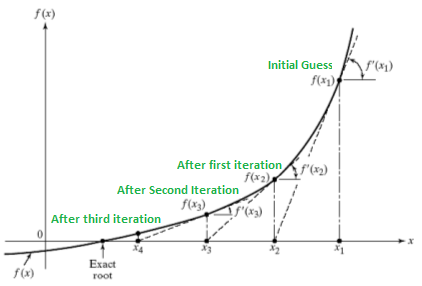
\includegraphics[width=0.8\linewidth]{NewtonRaphson}
			\caption{Visual depiction of the algorithm}
		\end{figure}
	\end{block}
	
\end{frame}

\begin{frame}	
	\frametitle{The Newton-Raphson Method}
	
	\begin{block}{Deriving Newton-Raphson:}
		
		\minipage{0.45\textwidth}
			Find the equation of the line from $f(x_1)$ to 0:
			\begin{equation*}
				\begin{split}
				y - \hat y & = m (x - \hat x) \\
				y - f(x_1) & = f'(x_1) (x - x_1) \\
				0 - f(x_1) & = f'(x_1) (x_2 - x_1) \\
				x_2 & = x_1 - \frac{f(x_1)}{f'(x_1)}
				\end{split}
			\end{equation*}
		\endminipage\hfill		
		\minipage{0.01\textwidth}
		\endminipage\hfill		
		\minipage{0.54\textwidth}
			\begin{figure}[ht]
				\centering
				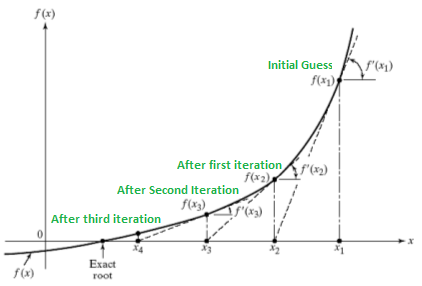
\includegraphics[width=0.95\linewidth]{NewtonRaphson}
%				\caption{Visual depiction of the algorithm}
			\end{figure}
		\endminipage\hfill
	\end{block}
	
\end{frame}


\begin{frame}	
	\frametitle{The Newton-Raphson Method}
	
	\begin{block}{The Newton-Raphson Method:}
		Solve $f(x) = x^2 - 2 = 0$ (i.e., find $\sqrt{2}$)
			
		\vspace{10pt}
		\minipage{0.5\textwidth}
			\begin{scriptsize}
			\code{c = 2 \\[-5pt]
			eps = 0.01 \\[-5pt]
			ans = 10 \\[-5pt]
			\tab \\[-5pt]
			while abs(ans**2 - c) >= eps: \\[-5pt]
			\tab ans = ans - (ans**2 - c)/(2*ans) \\[-5pt]
			\# end \\[-5pt]
			\tab \\[-5pt]
			print('sqrt(', c, ') is about', ans)
			}
			\end{scriptsize}
		\endminipage\hfill
		\minipage{0.5\textwidth}
			\begin{itemize}
				\item $f'(x) = 2x$
				\item The closer the initial guess is to the answer, the fewer steps required
				\item This function has multiple roots
			\end{itemize}
		\endminipage\hfill
	\end{block}
	
\end{frame}

\begin{frame}	
	\frametitle{The Newton-Raphson Method}
	
	\begin{block}{Limitations of Newton-Raphson:}
		
		\minipage{0.45\textwidth}
			\begin{itemize}
				\item Method can get stuck in a loop on certain functions
				\item If the method ever lands on $f'(x_i)=0$, then the method crashes due to a divide by zero error
			\end{itemize}
		\endminipage\hfill		
		\minipage{0.01\textwidth}
		\endminipage\hfill		
		\minipage{0.54\textwidth}
			\begin{figure}[ht]
				\centering
				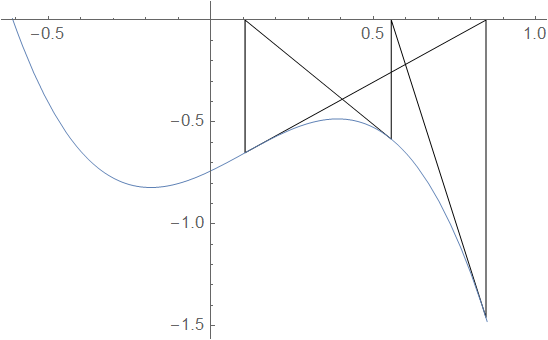
\includegraphics[width=0.7\linewidth]{NewtonRaphsonCubic} \\[10pt]
				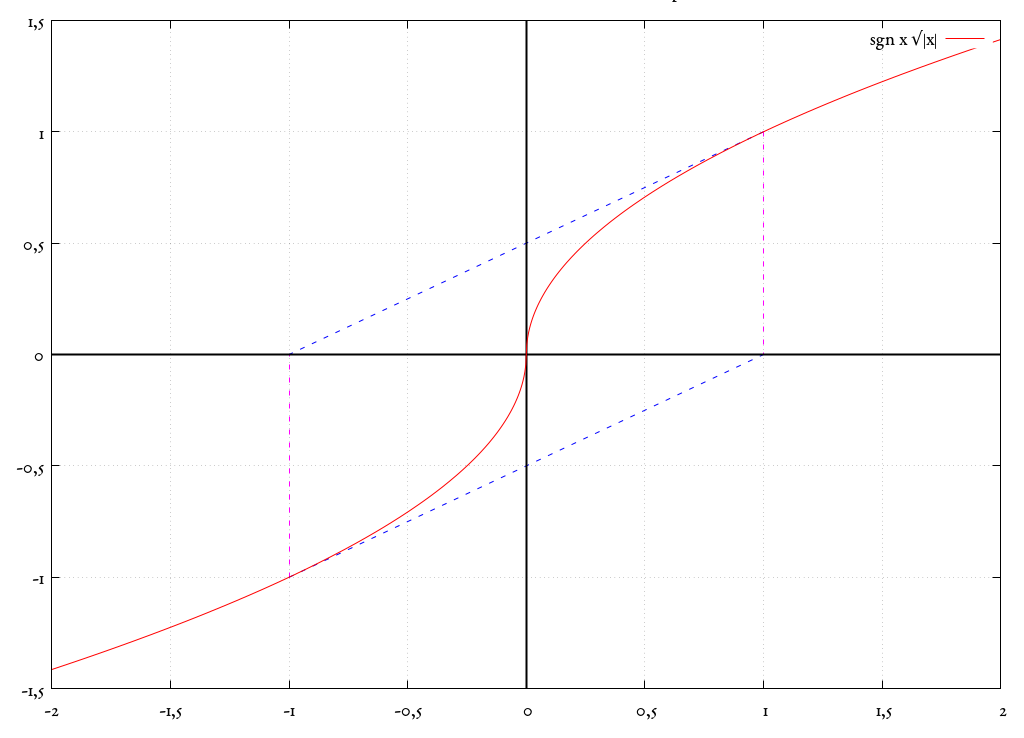
\includegraphics[width=0.7\linewidth]{NewtonRaphsonStuck}
%				\caption{Visual depiction of the algorithm}
			\end{figure}
		\endminipage\hfill
	\end{block}
	
\end{frame}

\begin{frame}	
	\frametitle{The Newton-Raphson Method}
	
	\begin{block}{3 methods compared:}
		Brute force (exhaustive elimination):
		\begin{itemize}
			\item Simple
			\item Most real-world cases have a search space way too large
		\end{itemize}
		Bisection:
		\begin{itemize}
			\item Far more efficient than brute force
			\item Needs search space to be ordered (many are, not a big deal)
			\item \code{high,low} values need to contain the answer between them
		\end{itemize}
		Newton-Raphson:
		\begin{itemize}
			\item Most efficient of all three
			\item Needs search space to be ordered (many are, not a big deal)
			\item Needs to evaluate derivative (in many real-world applications, this is non-trivial and computationally expensive)
			\item Method behaves poorly on certain functions
		\end{itemize}
	\end{block}
	
\end{frame}


 
\end{document}








